%-%-%-%-%-%-%-%-%-%-%-%-%-%-%-%-%-%-%-%-%-%-%-%-%-%-%-%-%-%-%-%-%-%-%-%-%-%-%
%%% MAIN DOCUMENT %%%

%-%-%-%-%-%-%-%-%-%-%-%-%-%-%-%-%-%-%-%-%-%-%-%-%-%-%-%-%-%-%-%-%-%-%-%-%-%-%

\documentclass[12pt, oneside]{book}
\usepackage{xcolor}
\usepackage{minted}

% \usepackage[T1]{fontenc}

\usepackage{draculatheme}
\newcommand{\documentTheme}{draculafg}
\newcommand{\documentLogo}{../../images/small logo_white.png}
\newcommand{\documentBigLogo}{../../images/logo_white_text.png}
\usemintedstyle{dracula}

\usemintedstyle{dracula}

\setminted{
    linenos=true,
    numbersep=5pt,
    frame=lines,
    framesep=2mm,
    breaklines=true
}

% \newcommand{\documentBigLogo}{../../images/Hendrix Logo.png}
% \newcommand{\documentLogo}{../../images/small logo.png}
% \newcommand{\documentTheme}{black}

%%% AESTHETICS %%%
%-%-%-%-%-%-%-%-%-%-%-%-%-%-%-%-%-%-%-%-%-%-%-%-%-%-%-%-%-%-%-%-%-%-%-%-%-%-%


%%% Dimensions and Spacing %%%
\usepackage[margin=1in]{geometry}
\setlength{\parindent}{0pt}
\usepackage{setspace}
\usepackage{mathtools}
\usepackage{esint}
\usepackage{adjustbox}
\linespread{1}
\usepackage{listings}
\usepackage{tikz}
\usetikzlibrary{shapes,backgrounds,calc,patterns,positioning}
\usepgflibrary{shadings}
\usepackage{pgfkeys}
\usepackage{pdftexcmds}
\usepackage{shellesc}
\usepackage{algorithm, algorithmic, xspace}
%%% Define new colors %%%
\definecolor{orangehdx}{rgb}{0.96, 0.51, 0.16}

% Normal colors
\definecolor{xred}{HTML}{BD4242}
\definecolor{xblue}{HTML}{4268BD}
\definecolor{xgreen}{HTML}{52B256}
\definecolor{xpurple}{HTML}{7F52B2}
\definecolor{xorange}{HTML}{FD9337}
\definecolor{xdotted}{HTML}{999999}
\definecolor{xgray}{HTML}{777777}
\definecolor{xcyan}{HTML}{80F5DC}
\definecolor{xpink}{HTML}{F690EA}
\definecolor{xgrayblue}{HTML}{49B095}
\definecolor{xgraycyan}{HTML}{5AA1B9}

% Dark colors
\colorlet{xdarkred}{red!85!black}
\colorlet{xdarkblue}{xblue!85!black}
\colorlet{xdarkgreen}{xgreen!85!black}
\colorlet{xdarkpurple}{xpurple!85!black}
\colorlet{xdarkorange}{xorange!85!black}
\definecolor{xdarkcyan}{HTML}{008B8B}
\colorlet{xdarkgray}{xgray!85!black}

% Very dark colors
\colorlet{xverydarkblue}{xblue!50!black}

% Document-specific colors
\colorlet{normaltextcolor}{black}
\colorlet{figtextcolor}{xblue}

% Enumerated colors
\colorlet{xcol0}{black}
\colorlet{xcol1}{xred}
\colorlet{xcol2}{xblue}
\colorlet{xcol3}{xgreen}
\colorlet{xcol4}{xpurple}
\colorlet{xcol5}{xorange}
\colorlet{xcol6}{xcyan}
\colorlet{xcol7}{xpink!75!black}

% Blue-Purple (should just used colorbrewer...)
\definecolor{xrainbow0}{HTML}{e41a1c}
\definecolor{xrainbow1}{HTML}{a24057}
\definecolor{xrainbow2}{HTML}{606692}
\definecolor{xrainbow3}{HTML}{3a85a8}
\definecolor{xrainbow4}{HTML}{42977e}
\definecolor{xrainbow5}{HTML}{4aaa54}
\definecolor{xrainbow6}{HTML}{629363}
\definecolor{xrainbow7}{HTML}{7e6e85}
\definecolor{xrainbow8}{HTML}{9c509b}
\definecolor{xrainbow9}{HTML}{c4625d}
\definecolor{xrainbow10}{HTML}{eb751f}
\definecolor{xrainbow11}{HTML}{ff9709}

%------- %
% XHFILL %
%------- %



%%% Chapter Headings %%%

\newcommand{\gradientrule}{
    \begin{tikzpicture}
        \shade[left color=orangehdx, right color=black, middle color=gray] (0,0) rectangle (\linewidth,0.4pt);
    \end{tikzpicture}
}

\usepackage[Glenn]{fncychap}
\ChTitleVar{\bfseries\scshape\color{\documentTheme}} % Needed for Dracula theme
\ChNumVar{\large\selectfont\color{\documentTheme}} % Needed for Dracula theme
\ChNameVar{\large\color{\documentTheme}} % Needed for Dracula theme
\usepackage{xpatch}


\xpatchcmd\DOCH
{\mghrulefill}{\color{orangehdx}\mghrulefill}
{}{\PatchFailed}
\xpatchcmd\DOTI
{\mghrulefill}{\color{orangehdx}\mghrulefill}
{}{\PatchFailed}
\xpatchcmd\DOTIS
{\mghrulefill}{\color{orangehdx}\mghrulefill}
{}{\PatchFailed}



%% Change Chapter Heading Placement %%
\usepackage{etoolbox}
\makeatletter
\patchcmd{\@makechapterhead}{\vspace*{50\p@}}{\vspace*{-20\p@}}{}{}
\patchcmd{\@makeschapterhead}{\vspace*{50\p@}}{\vspace*{-20\p@}}{}{}
\patchcmd{\DOTI}{\vskip 80\p@}{\vskip 40\p@}{}{}
\patchcmd{\DOTIS}{\vskip 40\p@}{\vskip 0\p@}{}{}
\makeatother



\renewcommand{\thesection}{\thechapter.\arabic{section}} %% Chapter.Section Numbering


%%% listingS %%%
\usepackage{graphicx}  
% \numberwithin{listing}{section}
\usepackage{float}
\usepackage{caption}

%%% Hyperlinks %%%
\usepackage{hyperref}
\definecolor{horange}{HTML}{f58026}
\hypersetup{
	colorlinks=true,
	linkcolor=horange,
	filecolor=horange,      
	urlcolor=horange,
}

\newcommand{\assignmentname}{Homework 4: Chapter 3 (Lin Alg)}

%% Headers and Footers %%
\usepackage{fancyhdr} % This should be set AFTER setting up the page geometry
\pagestyle{fancy} % options: empty , plain , fancy
\fancyhead[R]{\textcolor{draculafg}{\assignmentname}}
\fancyhead[L]{\textcolor{draculafg}{Hendrix College}}
\fancyhead[C]{\includegraphics[height=.50cm]{\documentLogo}} % Use for Dracula
\usepackage{xpatch}
\xpretocmd\headrule{\color{orangehdx}}{}{\PatchFailed}
\setlength{\footskip}{0.5in}
\setlength{\headheight}{18.5764pt}


%%%%% Colored Boxes %%%%%
\usepackage{tcolorbox}
\tcbuselibrary{skins}
\tcbuselibrary{theorems}
% \tcbuselibrary{minted}
\newcounter{BoxCounter}
\usepackage{dingbat}

%-%-%-%-%-%-%-%-%-%-%-%-%-%-%-%-%-%-%-%-%-%-%-%-%-%-%-%-%-%-%-%-%-%-%-%-%-%-%

%% MATH PACKAGES, ENVIRONMENTS, COMMANDS %%
%-%-%-%-%-%-%-%-%-%-%-%-%-%-%-%-%-%-%-%-%-%-%-%-%-%-%-%-%-%-%-%-%-%-%-%-%-%-%
%You'll need your own packages, theorem types, and commands.

\usepackage{fix-cm}
\usepackage{amsmath,amsthm} 
\usepackage{array, makecell}
\usepackage{colortbl}
\newcommand{\thickvrule}{\vrule width 1pt}

\newcommand{\thickhrule}{\Xhline{1pt}}

\usepackage{mathtools}
\usepackage{amssymb}
\usepackage[framemethod=tikz]{mdframed}
\usepackage{mathrsfs}
\usepackage{changepage}
\usepackage{multicol}
\usepackage{slashed}
\usepackage{enumerate}
\usepackage{braket}
\usepackage{booktabs}
\usepackage{enumitem}
\usepackage{kantlipsum}  %This package lets us generate random text for example purposes.
\usepackage{pgfplots}


%%% Custom Commands %%%
% Natural Numbers 
\newcommand{\N}{\mathbb{N}}

% Whole Numbers
\newcommand{\W}{\mathbb{W}}

% Integers
\newcommand{\Z}{\mathbb{Z}}

% Rational Numbers
\newcommand{\Q}{\mathbb{Q}}

% Real Numbers
\newcommand{\R}{\mathbb{R}}

% Complex Numbers
\newcommand{\C}{\mathbb{C}}

\newcommand{\I}{\mathbb{I}}

\newcommand{\pfs}{\noindent\makebox[\linewidth]{\rule{\textwidth}{0.4pt}}\vspace{0.5cm}}

\newcommand{\mysqrt}[1]{%
	\mathpalette\foo{#1}%
}
\newcommand{\dmysqrt}[1]{%
	\mathpalette\foodisplay{#1}%
}

% !TeX spellcheck = off
\newcommand{\foo}[2]{%
	% #1: math style, #2: content
	\sbox0{$#1\sqrt{#2}$}% Measure the size of the standard sqrt in the current style
	\begin{tikzpicture}[baseline=(sqrt.base)]
		\node[inner sep=0, outer sep=0] (sqrt) {$#1\sqrt{#2}$}; % Use the current math style
		\draw([yshift=-0.045em]sqrt.north east) -- ++(0,-0.5ex); % Draw the tick
	\end{tikzpicture}%
}
% !TeX spellcheck = off
\newcommand{\foodisplay}[2]{%
	% #1: math style, #2: content
	\sbox0{$#1\sqrt{#2}$}% Measure the size of the standard sqrt in the current style
	\begin{tikzpicture}[baseline=(sqrt.base)]
		\node[inner sep=0, outer sep=0] (sqrt) {$\displaystyle\sqrt{#2}$}; % Force displaystyle
		\draw[line width=0.4pt] ([yshift=-0.044em]sqrt.north east) -- ++(0,-0.5ex); % Draw the tick
	\end{tikzpicture}%
}

\renewcommand{\theenumi}{\arabic{enumi}}
\renewcommand{\labelenumi}{\textbf{\theenumi}.}
\renewcommand{\theenumii}{\alph{enumii}}
\renewcommand{\labelenumii}{\textbf{\theenumii}.}

% \newcommand{}{\marginnote{
\includegraphics[width=2em]{caution.png}}}

\newmdenv[
	topline=false,
	bottomline=true,
	rightline=false,
	leftline=true,
	linewidth=1.5pt,
	linecolor=black, % default color, will be overridden in custom commands
	backgroundcolor=draculabg, % Needed for Dracula theme
	fontcolor=\documentTheme, % Needed for Dracula theme
	innertopmargin=0pt,
	innerbottommargin=5pt,
	innerrightmargin=10pt,
	innerleftmargin=10pt,
	leftmargin=0pt,
	rightmargin=0pt,
	skipabove=\topsep,
	skipbelow=\topsep,
]{customframedproof}

\newenvironment{proofpart}[2][black]{
    \begin{mdframed}[
        topline=false,
        bottomline=false,
        rightline=false,
        leftline=true,
        linewidth=1pt,
        linecolor=#1!40, % Custom color
        % innertopmargin=10pt,
        % innerbottommargin=10pt,
        innerleftmargin=10pt,
        innerrightmargin=10pt,
        leftmargin=0pt,
        rightmargin=0pt,
        % skipabove=\topsep,
        % skipbelow=\topsep%
    ]
    \noindent
    \begin{minipage}[t]{0.08\textwidth}%
        \textbf{#2}%
    \end{minipage}%
    \begin{minipage}[t]{0.90\textwidth}%
        \begin{adjustwidth}{0pt}{0pt}%
}{
    \end{adjustwidth}
    \end{minipage}
    \end{mdframed}
}

% Define a new environment 'proofscratch' for Proof and Scratch Paper
\newenvironment{proofscratch}[2]{%
    \begin{mdframed}[
        topline=false,
        bottomline=false,
        rightline=false,
        leftline=false,
        backgroundcolor=draculabg, % Background color for Dracula theme
        fontcolor=\documentTheme,       % Font color for Dracula theme
        innerleftmargin=-6pt,
        innertopmargin=0pt,
        leftmargin=0pt,
        rightmargin=0pt,
        skipabove=\topsep,
        skipbelow=\topsep,
    ]
    % % Begin TikZ picture for the vertical dotted line
    % \begin{tikzpicture}[overlay, remember picture]
    %     % Draw a vertical dotted line at approximately the center of the mdframed width
    %     \draw[dotted, thick] ([xshift=0.005\linewidth]current bounding box.north west) -- ([xshift=0.005\linewidth]current bounding box.south west);
    % \end{tikzpicture}%
    % % Create the left minipage for Proof
    \begin{minipage}[t]{0.47\textwidth}%
        \noindent\textit{Proof.} #1 \hfill \(\qed\)
    \end{minipage}%
    \hfill
    % Create the right minipage for Scratch Paper
    \begin{minipage}[t]{0.47\textwidth}%
        \textit{Scratch Paper.} #2
    \end{minipage}%
}{
    \end{mdframed}
}

\newenvironment{tipbox}
	{%
		\par\noindent%
		% Top dashed line (using \textwidth)
		\tikz[baseline]{\draw[dash pattern=on 3pt off 2pt, line width=0.5pt, color=draculapurple] (0,0) -- (\textwidth,0);}%
		\par\vspace{0.65em}%
		\noindent\textbf{\textcolor{draculapurple}{TIP:}}\quad%
	}
	{%
		\par%
		% Bottom dashed line
		\noindent%
		\tikz[baseline]{\draw[dash pattern=on 3pt off 2pt, line width=0.5pt, color=draculapurple] (0,0) -- (\textwidth,0);}%
		\par\vspace{0.35em}
	}

\newenvironment{notebox}
	{%
		\par\noindent%
		% Top dashed line (using \textwidth)
		\tikz[baseline]{\draw[dash pattern=on 3pt off 2pt, line width=0.5pt, color=draculagreen] (0,0) -- (\textwidth,0);}%
		\par\vspace{0.65em}%
		\noindent\textbf{\textcolor{draculagreen}{NOTE:}}\quad%
	}
	{%
		\par%
		% Bottom dashed line
		\noindent%
		\tikz[baseline]{\draw[dash pattern=on 3pt off 2pt, line width=0.5pt, color=draculagreen] (0,0) -- (\textwidth,0);}%
		\par\vspace{0.35em}
	}

\newenvironment{warningbox}
	{%
		\par\noindent%
		% Top dashed line (using \textwidth)
		\tikz[baseline]{\draw[dash pattern=on 3pt off 2pt, line width=0.5pt, color=draculared] (0,0) -- (\textwidth,0);}%
		\par\vspace{0.65em}%
		\noindent\textbf{\textcolor{draculared}{WARNING:}}\quad%
	}
	{%
		\par%
		% Bottom dashed line
		\noindent%
		\tikz[baseline]{\draw[dash pattern=on 3pt off 2pt, line width=0.5pt, color=draculared] (0,0) -- (\textwidth,0);}%
		\par\vspace{0.35em}
	}

\newenvironment{solution}{\textit{Solution.}}

\newcommand{\sol}[1]{
    \begin{customframedproof}[linecolor=orangehdx!75,]
        \begin{solution}
        #1
        \end{solution}
    \end{customframedproof}
}

\newcommand{\pf}[1]{
    \begin{customframedproof}[linecolor=orangehdx!75]
        \begin{proof}
        #1
        \end{proof}
    \end{customframedproof}
}

\def \proofDistance {10pt}

\newcommand{\disabs}[1]{\ensuremath{\left|#1\right|}}
\newcommand{\limn}{\lim_{n \rightarrow \infty}}
\newcommand{\limx}[2]{\lim_{x \rightarrow #1}#2}

\newcommand{\limc}[1]{\lim_{x \rightarrow c}#1}

\newcommand{\ninn}{n \in \N}

\newcommand{\mb}[1]{\mathbf{#1}}

\newcommand{\limsupn}[1]{\limsup_{n\rightarrow \infty}#1}
\newcommand{\liminfn}[1]{\liminf_{n\rightarrow \infty}#1}


\newcommand{\proj}{\text{proj}}

\newcommand{\p}{\partial}

\newcommand{\dydx}{\frac{dy}{dx}}
\newcommand{\dxdy}{\frac{dx}{dy}}
\newcommand{\dydt}{\frac{dy}{dt}}
\newcommand{\dxdt}{\frac{dx}{dt}}
\newcommand{\dzdt}{\frac{dz}{dt}}

\newcommand{\barNotationT}[1]{\bigg|_{t = #1}}

\newcommand{\cyanit}[1]{\textit{\textcolor{cyan}{#1}}}

\newcommand{\brackett}[1]{\left\langle #1 \right\rangle}

\newcommand{\norm}[1]{\left\lVert \mathbf{#1}\right\rVert}

\newcommand{\imb}{\mb{i}}
\newcommand{\jmb}{\mb{j}}
\newcommand{\kmb}{\mb{k}}
\newcommand{\rmb}{\mb{r}}
\newcommand{\umb}{\mb{u}}

\newcommand{\vecfuc}[2]{\mb{#1}(#2)}
\newcommand{\dvecfuc}[2]{\mb{#1}'(#2)}
\newcommand{\normdvecfuc}[2]{\|\mb{#1}'(#2)\|}

\newcommand{\squigglyline}{%
    \noindent
    \tikz[baseline=-0.5ex]{
        \draw[decorate, decoration={snake, amplitude=0.5mm, segment length=3mm}] 
        (0,0) -- (\dimexpr\linewidth\relax,0);
    }%
}


% end of preamble
%-%-%-%-%-%-%-%-%-%-%-%-%-%-%-%-%-%-%-%-%-%-%-%-%-%-%-%-%-%-%-%-%-%-%-%-%-%-%

\begin{document}


%-%-%-%-%-%-%-%-%-%-%-%-%-%-%-%-%-%-%-%-%-%-%-%-%-%-%-%-%-%-%-%-%-%-%-%-%-%-%
%%% COVER PAGE %%%
%-%-%-%-%-%-%-%-%-%-%-%-%-%-%-%-%-%-%-%-%-%-%-%-%-%-%-%-%-%-%-%-%-%-%-%-%-%-%

% Do not use all caps.
\newcommand{\cussubtitle}{Mathematical Models}
% Date format should be like: "January 1, 2001"
\newcommand{\finaldate}{February 17, 2026}
% Be sure to include degree recognition (e.g., B.S., M.S., Ph.D)
\newcommand{\professor}{Dr. Christopher Camfield}

% -%-%-%-%-%-%-%-%-%-%-%-%-%-%-%-%-%-%-%-%-%-%-%-%-%-%-%-%-%-%-%-%-%-%-%-%-%-%

\begin{titlepage}
    \begin{center}

        \vspace*{-2cm}
        \includegraphics[width=0.8\textwidth]{\documentBigLogo}\\
        \vfill

        % Horizontal line above the title in 'horange' color
        \textcolor{horange}{\rule{\textwidth}{1.0pt}}

        \vspace{2em}

        {\huge \textbf{\assignmentname}}

        \vspace{1em} % Space between the title and the bottom line

        \textcolor{horange}{\rule{\textwidth}{1.0pt}}

        \vspace*{1\baselineskip}

        {\LARGE \textbf{\cussubtitle}}

        \begin{large}
            \vspace*{5\baselineskip}

            \vspace*{1\baselineskip}

            \emph{Author} \\[1ex]
            %Submitted by \\[\baselineskip]
            {\Large Paul Beggs \\ \par} % Editor list
            {\href{mailto:BeggsPA@Hendrix.edu}{{BeggsPA@Hendrix.edu}}}\\ % Editor affiliation

            \vspace*{1\baselineskip}

            \textit{Instructor} \\[1ex] % Tagline(s) or further description
            \professor

            \vspace*{1\baselineskip}

            \textit{Due}\\[1ex]
            {\scshape  \finaldate} \\[0.3\baselineskip] % Year published

            \thispagestyle{empty}

        \end{large}
    \end{center}
\end{titlepage}
% -%-%-%-%-%-%-%-%-%-%-%-%-%-%-%-%-%-%-%-%-%-%-%-%-%-%-%-%-%-%-%-%-%-%-%-%-%-%

% Chapter 3, Exercise 16ad, 18ac

\section*{Chapter 3}

\begin{enumerate}
    \setcounter{enumi}{15}
    \item A manufacturer of personal computers sells three desktop models. Model \(A\) costs \$850 to manufacture and sells for \$1,250; model \(B\) costs \$950 to manufacture and sells for \$1,400; and model \(C\) costs \$1,500 to manufacture and sells for \$2,500. The company purchases 10,000 desktop cases each month, and each computer requires one case. Models \(A\) and \(B\) use a 15–inch monitor, and the company can obtain 5,000 of these monitors per month. Model \(C\) uses a 17–inch monitor, and 7,500 of these are available per month. The remaining components are freely available. The company has 20,000 hours of production capacity available per month, and the production of each unit of model \(A\), \(B\), and \(C\) requires 1, 1.25, and 1.75 hours respectively. \hyperref[ex:1]{Excel Sheet}
    \begin{enumerate}
        \item How many of each type of computer should the company produce? Use the five-step method and solve as a linear programming problem.

        \sol{
            To maximize profits, the company should make 0 model \(A\)'s, 2,500 model \(B\)'s, and 7,500 model \(C\)'s to achieve a maximum monthly profit of \$8,625,000. It is also prudent to note that we have an additional 3,750 hours of production and 2,500 15-inch monitors available that we are not utilizing because we have a supply bottleneck of cases and 17-inch monitors. 
        }

        \setcounter{enumii}{3}

        \item The company is considering a new desktop model \(D\). This model will cost \$1,250 to manufacture and will sell for \$1,895. It requires a desktop case, a 17–inch monitor, and 1.5 hours of production. How will this change the results of parts (a) and (b)? Would you advise the company to go ahead with their plans to introduce this new model?

        \sol{
            We can advise the company with two arguments that approach the problem in different ways: 
            \begin{enumerate}[label=\arabic*)]
                \item \textbf{Modeling:} We can give them the results of running the program again with the addition of model \(D\), which outputs that the company should stick to 2,500 model \(B\)'s and 7,500 model \(C\)'s. Or, we could give them a logical argument that doesn't involve another round of computation.
                \item \textbf{Logic:} As mentioned in part (a), we have a bottleneck of cases and 17-inch monitors, with labor-hours and 15-inch monitors that are not being utilized because of the fact. Thus, adding a new model that requires less labor-hours, but also dips into the case and 17-inch monitor supply is not advisable, as it does not address the bottleneck. In addition, the profit for model \(C\) is \$1000, whereas model \(D\) is \$645. This shows that the company would experience a net loss of \$355 per unit if they produced model \(D\) over \(C\). Therefore, the company should not include the new model, as it is less profitable than model \(C\), while also providing no added benefit, as the company already has a glut of labor-hours. They can look to increase profits by maximizing the number of model \(C\)'s they produce, until the labor-hours constraint is met (assuming demands stays constant given an influx of only one model (worked for Nvidia though)).
            \end{enumerate}
        }

    \newpage
    \end{enumerate}
    \setcounter{enumi}{17}
    \item The Green Supply Company manufactures plastic grocery bags and milk jugs. The company can obtain 5,000 lbs of used plastic bags, 18,000 lbs of used plastic milk jugs, and 40,000 of industrial plastic scraps per week at a cost of \$18, \$12, and \$10 per 100 lbs respectively. The company has orders for 4,000 boxes of plastic bags and 80,000 milk jugs per week. One box of plastic bags requires 6 lbs of plastic, costs \$5 to manufacture, and sells for \$14. It costs \$9 and requires 14 lbs of plastic to make 100 milk jugs, and the jugs retail for \$20. The plastic bags must be at least 25\% post– consumer recycled plastic (used milk jugs or bags) because of consumer preference, and the milk jugs must be at most 50\% post–consumer recycled plastic for strength. \hyperref[ex:2]{Excel Sheet}
    \begin{enumerate}
        \item Determine the optimal mix of plastics for each product. Use the five-step method and model as a linear programming problem.
        \sol{
            We find the optimal mix of plastics to be 6,000 lbs of recycled plastic jugs and 29,200 lbs of plastic scrap. These values yield a profit of \$41,160 per week. Also, it's worth noting that we assumed the prices of \$18, \$12, and \$10 per 100 pounds could be changed to \$0.18, \$0.12, and \$0.1 per 1 pound. If it were the case that the company could only get those prices if they bought the plastic wholesale (i.e., only available in 100 lbs quantities), then the model would have to be slightly altered. 
        }
        \setcounter{enumii}{2}
        \item A new supplier can provide industrial plastic scraps at \$8 per 100 lbs. How does this change the results in parts (a) and (b)? 
        \sol{
            Given the new supplier, we would not change the amounts of plastic that we are ordering, as we are already maxing out the plastic scraps as it stands. The company would, however, experience have a profit increase of \$584. 
        }
    \end{enumerate}
\end{enumerate}

\newpage

\begin{figure}
\label{ex:1}
    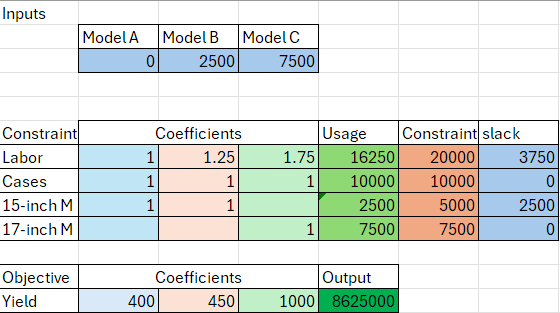
\includegraphics[width=\linewidth]{images/PB16a.png}
    \caption{Linear programming solution in Excel for Exercise 16}
\end{figure}


\newpage

\begin{figure}
\label{ex:2}
    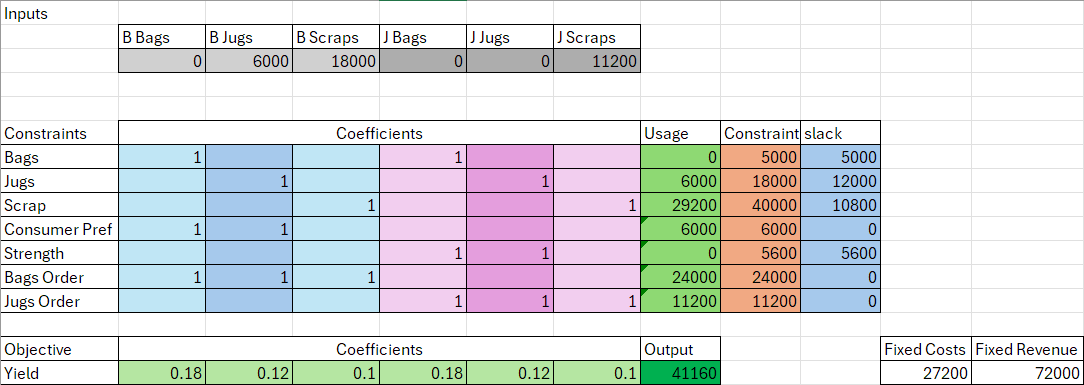
\includegraphics[width=\linewidth]{images/PB18a.png}
    \caption{Linear programming solution in Excel for Exercise 18}
\end{figure}


\end{document}